
%(BEGIN_QUESTION)
% Copyright 2008, Tony R. Kuphaldt, released under the Creative Commons Attribution License (v 1.0)
% This means you may do almost anything with this work of mine, so long as you give me proper credit

Identify what will happen to the output waveform from this amplifier circuit if resistor $R_1$ fails open, and explain why it will happen:

$$\includegraphics[width=15.5cm]{i03191x01.eps}$$

\vfil 

\underbar{file i03191}
\eject
%(END_QUESTION)





%(BEGIN_ANSWER)

This is a graded question -- no answers or hints given!

%(END_ANSWER)





%(BEGIN_NOTES)

With no $R_1$ providing a signal path to ground, the amplifier becomes a unity voltage follower.  We can tell this is the case by the fact that the inputs of an opamp draw negligible current, and in so doing the resistor R2 drops no voltage and behaves pretty much like a straight piece of wire as far as the opamp is concerned.  Thus, in doing it's job of maintaining the two input terminals at equal potential, the opamp duplicates the input voltage at its output terminal.

\vskip 10pt

Another way of looking at this is to see that an open resistor R1 causes the amplifier circuit to take on the form of a voltage follower.  Since we know voltage followers have a gain of 1, this tells us the amplifier will cause the output waveform to exactly follow the input waveform.

\vskip 10pt

A third way of looking at this is to recall that the overall gain of a non-inverting opamp circuit is ${R_{feedback} \over R_{ground}} + 1$.  When the resistance value of $R_{ground}$ goes to infinity, the overall gain approaches 1.  With a gain of 1, $V_{out}$ must equal $V_{in}$.

%INDEX% Electronics review: qualitative analysis of opamp amplifier circuit

%(END_NOTES)


